\documentclass[conference]{IEEEtran}
\IEEEoverridecommandlockouts
\usepackage[utf8]{inputenc}
\usepackage[T1]{fontenc}
\usepackage{cite}
\usepackage{amsmath,amssymb}
\usepackage{graphicx}
\usepackage{booktabs}
\usepackage{array}
\usepackage{tabularx}
\usepackage{xurl}
\usepackage{tikz}
\usetikzlibrary{arrows.meta,positioning,shapes.geometric,calc}
\usepackage{microtype}
\def\BibTeX{{\rm B\kern-.05em{\sc i\kern-.025em b}\kern-.08em T\kern-.1667em\lower.7ex\hbox{E}\kern-.125emX}}
\newcommand{\ck}{\checkmark}
\definecolor{navy}{RGB}{23,50,95}
\definecolor{teal}{RGB}{0,128,128}
\definecolor{amber}{RGB}{214,137,16}
\definecolor{softblue}{RGB}{232,240,250}
\definecolor{softred}{RGB}{252,232,230}
\definecolor{softgreen}{RGB}{230,245,236}

\begin{document}

\title{Cloud Forensics Challenges in Bangladesh:\\
A PRISMA-Guided Review with AI-Assisted\\ Resolution Strategies}

\author{\IEEEauthorblockN{Md. Ahsan Kabir}
\IEEEauthorblockA{\textit{Department of Computer Science and Engineering}\\
\textit{United International University, Dhaka, Bangladesh}\\
mkabir2520016@mscse.uiu.ac.bd}}

\maketitle

\begin{abstract}
Since 2023 Bangladesh has replaced its main cyber law twice, and its first data protection ordinance was replaced by an Act within six months, yet none of the new texts clearly tells a cloud provider to freeze logs for an investigator. This paper reviews 15 open-access studies with the PRISMA 2020 method and reads the primary legal texts on the government's law portal. We group the findings into five challenge clusters: short-lived data, shared infrastructure, chain of custody, cross-border access, and forensic readiness. The Cyber Security Act 2026 gives investigators a 90-day data preservation order (extendable to 180 days), a duty on service providers to help, and a rule that forensic evidence it covers is accepted as evidence, mostly carried over from the 2023 Act. But the preservation order names only the ``person or body in charge of the computer system'', and we found no rule on how Section 65B certificates should work for cloud records. The earlier requirement to keep a copy of restricted cloud data inside Bangladesh did not survive into the final data protection Act. We then match each cluster to tools reported in the literature, such as LLM-based log analysis and open-source law enforcement request management, and sketch a roadmap, AI-CFRF-BD. The roadmap is a proposal and has not been tested in Bangladesh.
\end{abstract}

\begin{IEEEkeywords}
cloud forensics, digital evidence, Bangladesh cyber law, PRISMA, forensic readiness, chain of custody
\end{IEEEkeywords}

\section{Introduction}
Government offices, banks and private firms in Bangladesh now keep many records on cloud platforms, and some of those platforms run outside the country. When a crime touches such records, an investigator faces three practical problems. The data may be deleted before anyone asks for it. A court may doubt that the copy shown is genuine. And the company holding it may answer to another country's law.

The problem is easy to underestimate because the first one is largely a matter of defaults. As one example, AWS CloudTrail shows 90 days of management events in its event history unless a customer sets up longer storage~\cite{aws}. If a case reaches a police station after that window, the account owner may have no copy at all. Other vendors set their own defaults, so an investigator cannot assume a standard period.

Bangladesh's legal framework has also moved quickly. The Cyber Security Act 2023 was repealed in May 2025, and Parliament passed a new Cyber Security Act in April 2026~\cite{cyberact}. The Personal Data Protection Ordinance 2025 was replaced by an Act in the same month~\cite{pdpa}. A study written around the 2023 law alone is now out of date.

\subsection{Research gap}
Global reviews describe cloud forensic challenges well~\cite{alshabibi,alenezi,prakash}. Bangladeshi studies describe weak investigation practice and legal gaps~\cite{ali,uzzal,ahmed,sharmin,rana}. We did not find a study that lines up the global cloud challenges against Bangladesh's current statutes, using the 2025--2026 texts, and then asks which tools reported in the literature could help. This paper tries to do that.

\subsection{Research questions}
\begin{itemize}
\item \textbf{RQ1.} What technical challenges do cloud environments create for digital forensics?
\item \textbf{RQ2.} What do Bangladesh's current laws say about cloud evidence, and where are the gaps?
\item \textbf{RQ3.} Which AI-assisted or automated tools in the literature address these challenges?
\item \textbf{RQ4.} What practical roadmap follows for Bangladeshi law enforcement?
\end{itemize}

\subsection{Contributions}
(i) A PRISMA-guided review of 15 studies (Table~\ref{tab:studies}). (ii) A primary-source map of Bangladesh's cyber, evidence and data protection laws from 2018 to 2026 (Fig.~\ref{fig:timeline}, Table~\ref{tab:laws}). (iii) A five-cluster challenge table that sets each cluster against the law and against tools from the literature (Table~\ref{tab:matrix}). (iv) A roadmap, AI-CFRF-BD, clearly labelled as a proposal (Fig.~\ref{fig:framework}).

\section{Related Work}
\subsection{Global cloud forensics}
Alshabibi et al.\ reviewed 20 studies and sorted the challenges they found into technical (42\%), resource (30\%) and legal (28\%) groups, noting that some challenges fit more than one group~\cite{alshabibi}. Prakash et al.\ add that in cloud and edge settings investigators often do not know where the evidence physically sits, and that the legal difficulties include authentication, hearsay, chain of custody and preservation~\cite{prakash}. Alenezi lists data acquisition, analysis, preservation, privacy and legal issues~\cite{alenezi}.

On the legal side, Karagiannis and Vergidis name three problems: territoriality (loss of location), possession (who owns cloud content) and the confiscation procedure. They then discuss and endorse the ``Power of Disposal'', a newly formed legal notion offered as a first step towards easing these problems~\cite{karagiannis}. Ekwempu focuses on jurisdiction, data sovereignty and admissibility in cross-border cases~\cite{ekwempu}. Akilal and Kechadi report that a formal Mutual Legal Assistance Treaty (MLAT) request takes from six weeks to ten months on average, a figure they take from earlier work~\cite{akilal}.

\subsection{Tools}
Alharthi and Garcia built CIAF, an ontology-driven framework that uses a large language model to analyse cloud logs. In a test on Microsoft Azure logs with ransomware-related events they report precision, recall and F1 of about 93\%~\cite{ciaf}. Akilal and Kechadi built a proof of concept for managing law enforcement requests from open-source parts and tested it in two scenarios~\cite{akilal}. K\"ulper et al.\ propose an acquisition framework for self-hosted storage such as Nextcloud, using the platform's own APIs~\cite{kulper}. Two reviews cover blockchain for evidence handling~\cite{igonor} and machine learning for forensic investigation in smart environments~\cite{tageldin}. None of these reports a test in Bangladesh.

\subsection{Bangladesh}
Ali observed in 2018 that Bangladesh lacked a full guideline for digital forensic investigators, and proposed a seven-phase evidence management framework~\cite{ali}. Uzzal's 2025 monograph lists legal ambiguity, procedural gaps, limited forensic capacity, weak inter-agency coordination and low awareness~\cite{uzzal}. Ahmed and Arifuzzaman find that existing law still protects users and data poorly and compare it with the GDPR and the Budapest Convention~\cite{ahmed}. Sharmin and Rahman surveyed 52 police members and recommend more training and technology~\cite{sharmin}. Rana compares investigation practice in Colombia, India and the United States and draws lessons for Bangladesh~\cite{rana}.

\section{Methodology}
We followed the PRISMA 2020 statement~\cite{prisma}. Four research questions were set before the search. The search used seven sources: arXiv (cs.CR), MDPI, Google Scholar, SSRN, the NDC e-Journal, the Bangladesh Journal of MIS and IJRIAS. Six query strings were applied: ``cloud forensics'', ``digital evidence Bangladesh'', ``AI forensics cloud'', ``blockchain digital forensics'', ``blockchain chain-of-custody'' and ``cyber law BD''. The window was 2021--2026, which covers recent cloud forensics work and the legal changes described in Section~IV.

\begin{figure}[t]
\centering
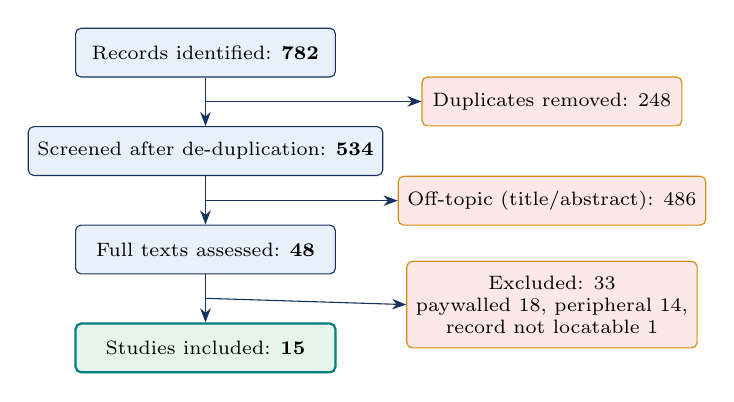
\begin{tikzpicture}[x=1cm,y=1cm,font=\scriptsize,
 box/.style={draw=navy,fill=softblue,rounded corners=2pt,minimum width=3.3cm,minimum height=0.62cm,align=center},
 ex/.style={draw=amber,fill=softred,rounded corners=2pt,minimum width=3.3cm,minimum height=0.62cm,align=center},
 ok/.style={draw=teal,fill=softgreen,rounded corners=2pt,minimum width=3.3cm,minimum height=0.62cm,align=center,thick},
 arr/.style={-{Stealth[length=1.8mm]},navy}]
\node[box] (a) at (0,0) {Records identified: \textbf{782}};
\node[box] (b) at (0,-1.25) {Screened after de-duplication: \textbf{534}};
\node[box] (c) at (0,-2.5) {Full texts assessed: \textbf{48}};
\node[ok]  (d) at (0,-3.75) {Studies included: \textbf{15}};
\node[ex] (a2) at (4.4,-0.62) {Duplicates removed: 248};
\node[ex] (b2) at (4.4,-1.88) {Off-topic (title/abstract): 486};
\node[ex,minimum height=1.1cm] (c2) at (4.4,-3.2) {Excluded: 33\\paywalled 18, peripheral 14,\\record not locatable 1};
\draw[arr] (a)--(b); \draw[arr] (b)--(c); \draw[arr] (c)--(d);
\draw[arr] (0,-0.62)--(a2.west); \draw[arr] (0,-1.88)--(b2.west);
\draw[arr] (0,-3.12)--(c2.west);
\end{tikzpicture}
\caption{PRISMA 2020 flow of the literature search.}
\label{fig:prisma}
\end{figure}

Of 782 records, 248 were duplicates. Screening the other 534 by title and abstract removed 486 as off-topic. Of 48 full texts, 18 were behind a paywall, 14 were only loosely connected to the five clusters, and one cited chapter could not be located in any catalogue, so we excluded it. That left 15 studies (Fig.~\ref{fig:prisma}). A paper was included if it addressed at least one challenge area from RQ1 or RQ2, was published in 2021--2026, was open access and was in English. We left out paywalled work so that readers can check every claim, but this also means we may have missed relevant studies.

One reviewer coded each study with the thematic synthesis steps of Thomas and Harden~\cite{thomas}: which cluster it addresses, whether Bangladesh is covered, and whether a tool is proposed. There was no second coder, so the cluster labels in Table~\ref{tab:studies} are our judgement and should be read that way.

For each study we also recorded its type (review, experiment, proof of concept, survey or position paper) and where any tool was tested. We did not use a formal quality score. Instead, we treated reviews and proofs of concept as weaker support for a claim that a tool works than a controlled experiment, and we say so in Section~VI.

Statutes are not counted among the 15 studies. We read the legal texts directly on the Bangladesh Laws portal in October 2026, in Bengali, and note section numbers so that others can check them. We make no claim to give legal advice.

\begin{table*}[t]
\centering
\caption{The 15 included studies. Design and status follow each paper's own description; clusters (C1--C5) were assigned by the author.}
\label{tab:studies}
\small
\renewcommand{\arraystretch}{1.08}
\begin{tabularx}{\textwidth}{@{}l l X l l c@{}}
\toprule
Ref. & Year & What the study reports & Design (status) & Clusters & BD \\
\midrule
\cite{alshabibi} & 2024 & Systematic review of 20 studies; challenges split 42\% technical, 30\% resource, 28\% legal & Systematic review (journal) & C1--C4 & -- \\
\cite{alenezi} & 2023 & Review of acquisition, analysis, preservation, privacy and legal challenges & Literature review (preprint) & C1, C2, C4 & -- \\
\cite{prakash} & 2021 & Cloud and edge forensics; unknown evidence location; legal issues of authentication, hearsay, custody & Review (journal) & C1, C3 & -- \\
\cite{ali} & 2018 & No full guideline for investigators; seven-phase evidence management framework & Framework proposal (journal) & C3, C5 & \ck \\
\cite{uzzal} & 2025 & Monograph on legal ambiguity, procedural gaps, weak capacity and coordination & Monograph (SSRN) & C3, C5 & \ck \\
\cite{ahmed} & 2025 & Legislative gaps in cybersecurity and data privacy; compares GDPR and Budapest Convention & Legal analysis (journal) & C4, C5 & \ck \\
\cite{sharmin} & 2025 & Survey of 52 police members; six impact dimensions; calls for training and technology & Survey, n=52 (journal) & C5 & \ck \\
\cite{rana} & 2025 & Comparative study of investigation reforms in Colombia, India and the United States & Comparative study (journal) & C3, C5 & \ck \\
\cite{karagiannis} & 2021 & Three legal challenges (territoriality, possession, confiscation); Power of Disposal & Legal analysis (journal) & C3, C4 & -- \\
\cite{ekwempu} & 2026 & Legal complexity of cross-border cloud investigations; data sovereignty, admissibility & Legal analysis (journal) & C4 & -- \\
\cite{akilal} & 2025 & Open-source law enforcement request management, proof of concept, two scenarios, cost estimate & Proof of concept (preprint) & C4, C5 & -- \\
\cite{ciaf} & 2025 & LLM and ontology framework for cloud logs; about 93\% F1 on Azure ransomware events & Experiment (preprint) & C1 & -- \\
\cite{kulper} & 2025 & Acquisition framework and open-source tool for self-hosted storage (Nextcloud) & Framework and tool (preprint) & C5 & -- \\
\cite{igonor} & 2025 & Literature review of blockchain in digital forensics (evidence integrity, custody) & Systematic review (journal) & C3 & -- \\
\cite{tageldin} & 2023 & Review of machine learning for forensic investigation in smart environments & Review (journal) & C1, C2 & -- \\
\bottomrule
\end{tabularx}
\end{table*}

\section{Bangladesh's Legal Position, 2018--2026}
\subsection{How the laws changed}
Fig.~\ref{fig:timeline} shows the sequence. The ICT Act 2006 set up the Cyber Tribunal (section 68) and the Cyber Appellate Tribunal (section 82)~\cite{cyberact}. The Digital Security Act 2018 let the Digital Security Agency order a computer system's managers to keep data for 90 days, with an extension through the Tribunal~\cite{unodc}. The Evidence (Amendment) Act 2022 (Act 20 of 2022, dated 20 November 2022) inserted sections 65A and 65B, which route the proof of digital records through a certificate from ``a person occupying a responsible official position''~\cite{evidence}. The Cyber Security Act 2023~\cite{act2023} was then repealed by the Cyber Protection Ordinance 2025 (21 May 2025)~\cite{ordinance}, which Parliament replaced with Act 81 of 2026, deemed in force from the same May date~\cite{cyberact}. An amending Act of 1 July 2026 (Act 99 of 2026) removes section 20 and nothing else~\cite{amend}. The official English title of Act 81 is not stated on the Bengali page we read; the Bengali title uses the word for ``protection'', and we call it the Cyber Security Act 2026, as most sources do.

\begin{figure*}[t]
\centering
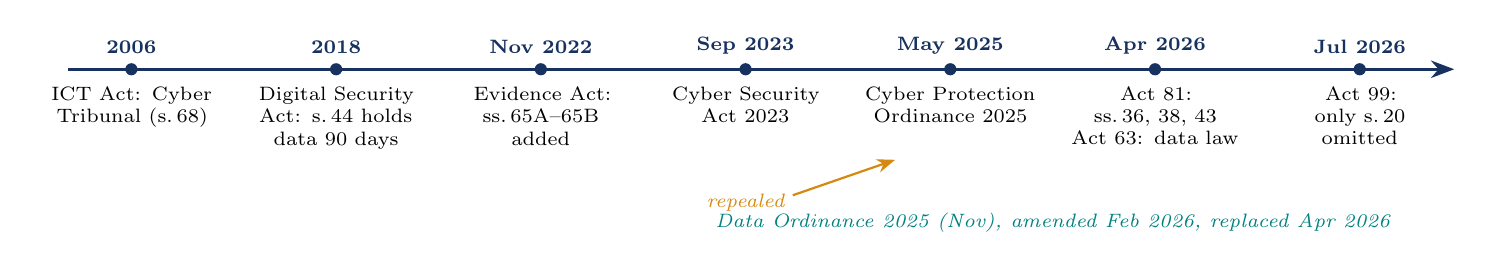
\begin{tikzpicture}[x=1cm,y=1cm,font=\scriptsize]
\draw[navy,very thick,-{Stealth}] (0,0)--(17.6,0);
\foreach \x/\lab/\tp in {0.8/2006/{ICT Act: Cyber\\Tribunal (s.\,68)},
 3.4/2018/{Digital Security\\Act: s.\,44 holds\\data 90 days},
 6.0/{Nov 2022}/{Evidence Act:\\ss.\,65A--65B\\added},
 8.6/{Sep 2023}/{Cyber Security\\Act 2023},
 11.2/{May 2025}/{Cyber Protection\\Ordinance 2025},
 13.8/{Apr 2026}/{Act 81:\ ss.\,36, 38, 43\\Act 63: data law},
 16.4/{Jul 2026}/{Act 99:\\only s.\,20\\omitted}}
 {\fill[navy] (\x,0) circle (2.2pt);
  \node[above=2pt,font=\scriptsize\bfseries,navy] at (\x,0) {\lab};
  \node[below=3pt,align=center,text width=2.4cm] at (\x,0) {\tp};}
\node[amber,font=\scriptsize\itshape] at (8.6,-1.7) {repealed};
\draw[amber,thick,-{Stealth}] (9.2,-1.6)--(10.5,-1.15);
\node[teal,font=\scriptsize\itshape] at (12.5,-1.95) {Data Ordinance 2025 (Nov), amended Feb 2026, replaced Apr 2026};
\end{tikzpicture}
\caption{Timeline of the main Bangladeshi laws that touch cloud evidence.}
\label{fig:timeline}
\end{figure*}

\subsection{Personal data law}
The Personal Data Protection Ordinance 2025 (Ordinance 61 of 2025) said in section 29(7), as replaced in February 2026, that restricted personal data and critical information infrastructure data must have at least one synchronised real-time copy in Bangladesh. It also let the Authority order a cloud arrangement changed or ended within 60 days if it endangered national interest or public safety~\cite{pdpo}. The final Personal Data Protection Act 2026 (Act 63 of 2026) does not contain either rule. Its section 29(7) only lets the Authority make regulations~\cite{pdpa}. We did not find a stated reason, so readers should not assume the idea was dropped for good.

What the Act does keep matters to investigators. Section 24(1) allows processing without consent to comply with a court order or to prevent, detect, investigate or prosecute an offence, though section 24(2) says other duties still apply. Section 20 requires a breach likely to cause significant harm to be reported to the Authority, with the time limit left to regulations. Section 29(6) requires notice to the Authority before large transfers abroad of sensitive identifiers such as ID, biometric and genetic data. Section 8 keeps a data fiduciary responsible for any processor it hires~\cite{pdpa}.

\subsection{What the Cyber Security Act 2026 gives investigators}
Table~\ref{tab:laws} lists the provisions that matter most. Five of them are directly useful for cloud work. Section 36 lets the Director General order data to be kept for 90 days, extendable by the Tribunal to a total of 180 days. Section 33 lets investigators take control of computers and stored data and collect traffic data. Section 34 allows a warrant covering traffic data held by a service provider. Section 38 says any person, body or service provider asked to help ``is bound'' to give information and assistance. Section 43 says forensic evidence obtained under the Act counts as evidence even if the Evidence Act of 1872 says otherwise, and requires digital forensic evidence prepared in a forensic lab to be preserved~\cite{cyberact}. The definition of ``cyber protection'' in section 2 names data centres and the cloud.

Most of this is not new. The 2023 Act already held the same 90-day order with a 180-day cap (s.\,43), the same duty to assist (s.\,45), the same rule on the evidential value of forensic evidence (s.\,56) and a rule-making clause that lists ``cloud computing, metadata'' (s.\,58)~\cite{act2023}. Table~\ref{tab:carry} sets them side by side. What the 2026 Act adds is the duty to keep digital forensic evidence prepared in a lab, and a wider wording of the cloud clause. In other words, cloud forensics has been named in Bangladeshi cyber law since 2023, but the powers around it were written for ordinary computers and carried forward unchanged.

\begin{table}[t]
\centering
\caption{Provisions of Act 81 of 2026 that bear on cloud evidence~\cite{cyberact}.}
\label{tab:laws}
\small
\renewcommand{\arraystretch}{1.05}
\begin{tabularx}{\columnwidth}{@{}l X@{}}
\toprule
Section & Content \\
\midrule
s.\,4 & Offence from abroad using a computer or network in Bangladesh is treated as committed in Bangladesh \\
s.\,33 & Investigator may take control of devices and data; collect traffic data \\
s.\,34 & Warrant (Tribunal or magistrate) can cover traffic data held by a service provider \\
s.\,36 & Preservation order, 90 days, up to 180 with Tribunal \\
s.\,38 & Duty on any person, body or service provider to assist \\
s.\,41 & Cyber Tribunal has sole jurisdiction over offences under the Act \\
s.\,43 & Forensic evidence under the Act counts as evidence; lab-prepared digital evidence must be kept \\
s.\,49(2) & Rules may be made on ``digital forensic matters related to cloud computing or metadata'' \\
\bottomrule
\end{tabularx}
\end{table}

\begin{table}[t]
\centering
\caption{Provisions carried from the 2023 Act into Act 81 of 2026~\cite{act2023,cyberact}.}
\label{tab:carry}
\small
\renewcommand{\arraystretch}{1.05}
\begin{tabularx}{\columnwidth}{@{}l l l@{}}
\toprule
Topic & 2023 Act & Act 81 (2026) \\
\midrule
Preservation, 90 + up to 180 days & s.\,43 & s.\,36 \\
Duty of providers to assist & s.\,45 & s.\,38 \\
Forensic evidence counts as evidence & s.\,56 & s.\,43 \\
Rules on cloud computing and metadata & s.\,58 & s.\,49(2) \\
Lab-prepared evidence must be kept & not found & s.\,43 \\
\bottomrule
\end{tabularx}
\end{table}

\subsection{What is still open}
First, the preservation order in section 36 is addressed to ``the person or body in charge of the computer or computer system''. It does not say whether a foreign cloud company counts, or how an order would reach it. Section 4 covers offences, not evidence on foreign servers, and the duty in section 38 has no stated way to be enforced abroad. Second, section 65B(4) was written with a single computer in mind; we found no model certificate or guidance for cloud records, where the ``responsible official'' might sit with the provider. Third, section 49(2) allows rules on cloud forensics and on how traffic data is collected, but the NCSA's list of laws shows no rules issued under the 2026 Act, or under the 2023 Act that had a similar clause~\cite{ncsa}. Fourth, Bangladesh's Mutual Legal Assistance in Criminal Matters Act 2012 names the Ministry of Home Affairs as the central authority~\cite{mha}; this is the route for foreign requests, with the delays noted in Section~II. We did not find a record of Bangladesh as a party to the Budapest Convention, and Ahmed and Arifuzzaman compare Bangladeshi law with it~\cite{ahmed}.

\section{Findings: Five Challenge Clusters}
\textbf{C1. Short-lived data.} One major provider's default is 90 days~\cite{aws}, and investigators often do not know where data sits~\cite{prakash}. Bangladesh has a preservation order, but it needs someone to notice the case in time and to know which provider to address.

\textbf{C2. Shared infrastructure.} Many customers share one platform, and the review literature links this to privacy limits and to the difficulty of separating one tenant's data from another's~\cite{alshabibi,alenezi}. The Personal Data Protection Act lets processing go ahead for an investigation, but other duties remain (s.\,24(2)). We found no Bangladeshi rule on how to handle shared evidence.

\textbf{C3. Chain of custody and admissibility.} Sections 65A--65B give the route into court; Act 81 s.\,43 adds weight for forensic evidence under that Act. Ali noted in 2018 that no complete guideline existed for investigators~\cite{ali}, and Uzzal's 2025 monograph still reports procedural gaps~\cite{uzzal}. For cloud records the missing piece is practical: who signs the certificate and what it says. Section 65B(2) asks the court to be satisfied that the computer was regularly used for the relevant activity, that the information was regularly fed into it, that it was working properly, and that the record reproduces what was fed in; section 65B(4) lets a responsible official certify this~\cite{evidence}. For a single office computer, the person who ran it can say so. For a cloud service, only the provider can speak to how the platform logs and stores data, so a certificate from the account holder may not be enough. This is our reading and has not been tested before the Tribunal.

\textbf{C4. Cross-border access.} Section 4 and the duties in sections 36 and 38 apply in Bangladesh, but the data may not be. MLAT requests take from six weeks to ten months~\cite{akilal}. Karagiannis and Vergidis describe the same loss of location as a legal problem in itself~\cite{karagiannis}.

\textbf{C5. Forensic readiness.} A police survey of 52 members found that digital forensics helps with evidence accuracy, collection procedure and conviction rates, and recommends training and technology~\cite{sharmin}. Rana's comparative study draws lessons on investigative effectiveness and the integrity of evidence~\cite{rana}. Government workloads that move to a locally hosted cloud, such as the sovereign cloud announced by the state data centre company~\cite{oracle}, would make local acquisition easier, but that applies only to workloads placed there.

\begin{table*}[t]
\centering
\caption{Challenge clusters set against Bangladesh's law and tools reported in the literature. Tool results are as reported by the authors, from other settings.}
\label{tab:matrix}
\small
\renewcommand{\arraystretch}{1.1}
\begin{tabularx}{\textwidth}{@{}l >{\raggedright\arraybackslash}p{2.6cm} >{\raggedright\arraybackslash}X >{\raggedright\arraybackslash}X >{\raggedright\arraybackslash}X@{}}
\toprule
 & Challenge & What Bangladesh law offers (2026) & Gap we found & Tool reported in the literature \\
\midrule
C1 & Short-lived data & Act 81 s.\,36: 90 + 90 days order; s.\,38 duty to assist & Order addressed to person in charge of the system; foreign providers not mentioned & CIAF: LLM log triage, about 93\% F1 on Azure ransomware test~\cite{ciaf} \\
C2 & Shared infrastructure & PDPA s.\,24: processing allowed for investigations; s.\,8 processor liability & No rule on separating tenants or handling mixed data & ML for large, mixed data in smart environments (review only)~\cite{tageldin} \\
C3 & Chain of custody; admissibility & Evidence Act 65A--65B; Act 81 s.\,43; forensic labs (ss.\,10--11) & No cloud certificate model; lab capacity unclear & Blockchain custody logs (review of designs, no field results)~\cite{igonor} \\
C4 & Cross-border access & Act 81 ss.\,4, 34, 38; MLA Act 2012; PDPA s.\,29(6) transfer notice & No direct provider channel; slow MLAT~\cite{akilal} & Request-management system, open source, two scenarios~\cite{akilal} \\
C5 & Forensic readiness & Act 81 s.\,49(2) allows cloud forensic rules; PDPA s.\,20 breach notice & No rules issued that we could find; training gaps~\cite{sharmin} & API-based acquisition for self-hosted storage~\cite{kulper} \\
\bottomrule
\end{tabularx}
\end{table*}

\section{AI-Assisted Strategies and a Roadmap}
We looked for tools in the literature that match each cluster (Table~\ref{tab:matrix}). Three points need to be clear. First, the numbers come from the authors' own tests, such as the Azure log experiment for CIAF~\cite{ciaf}, not from Bangladesh. Second, two of the five (blockchain and machine learning) are reviews of designs, not tested systems~\cite{igonor,tageldin}. Third, none of these tools replaces the legal steps. An AI-produced finding is a lead for a human investigator; the evidence that goes to court is still the original log with its hash and certificate.

\begin{table}[t]
\centering
\caption{Proposed pilot measures for AI-CFRF-BD.}
\label{tab:eval}
\small
\renewcommand{\arraystretch}{1.05}
\begin{tabularx}{\columnwidth}{@{}l X@{}}
\toprule
Cluster & Measure (against the manual baseline) \\
\midrule
C1 & Time from complaint to preservation order; share of cases where the log window had already closed \\
C2 & Share of tenant-mixed records correctly sorted, checked by a human analyst \\
C3 & Share of exhibits accepted with their certificate; hash mismatches found \\
C4 & Days to first provider response; MLAT requests sent and answered \\
C5 & Staff trained; checklist used in what share of new cases \\
All & Precision and recall of tool findings; analyst hours saved; errors that a human reviewer had to correct \\
\bottomrule
\end{tabularx}
\end{table}

\begin{table}[t]
\centering
\caption{How strong is the evidence for each tool? (as reported by the authors)}
\label{tab:maturity}
\small
\renewcommand{\arraystretch}{1.05}
\begin{tabularx}{\columnwidth}{@{}l l X@{}}
\toprule
Tool & Level & What was actually done \\
\midrule
CIAF~\cite{ciaf} & Experiment & Azure logs with simulated ransomware events; about 93\% precision, recall and F1 \\
Request system~\cite{akilal} & Proof of concept & Two realistic scenarios and a cost estimate; no field use \\
Nextcloud kit~\cite{kulper} & Framework and tool & Case study of one self-hosted platform \\
Blockchain~\cite{igonor} & Literature review & Designs compared; no performance results \\
ML in forensics~\cite{tageldin} & Literature review & Smart (IoT) settings, not cloud logs \\
\bottomrule
\end{tabularx}
\end{table}

\begin{figure}[t]
\centering
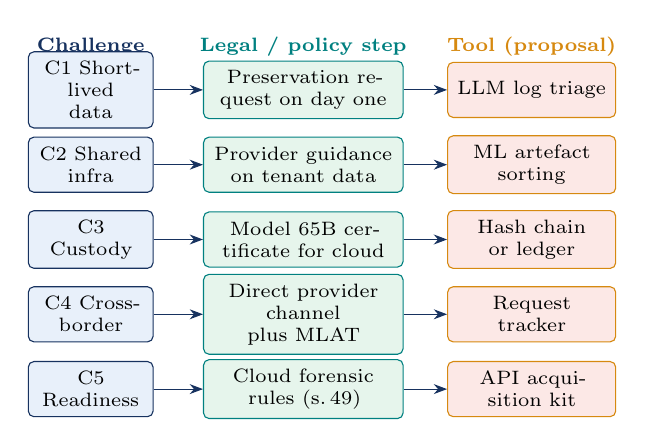
\begin{tikzpicture}[x=1cm,y=1cm,font=\scriptsize,
 blk/.style={draw=navy,fill=softblue,rounded corners=2pt,minimum height=0.7cm,text width=1.35cm,align=center},
 fix/.style={draw=teal,fill=softgreen,rounded corners=2pt,minimum height=0.7cm,text width=2.3cm,align=center},
 tl/.style={draw=amber,fill=softred,rounded corners=2pt,minimum height=0.7cm,text width=1.9cm,align=center}]
\node[font=\scriptsize\bfseries,navy] at (0.7,0.55) {Challenge};
\node[font=\scriptsize\bfseries,teal] at (3.4,0.55) {Legal / policy step};
\node[font=\scriptsize\bfseries,amber] at (6.3,0.55) {Tool (proposal)};
\foreach \i/\c/\f/\t in {0/{C1 Short-lived data}/{Preservation request on day one}/{LLM log triage},
 1/{C2 Shared infra}/{Provider guidance on tenant data}/{ML artefact sorting},
 2/{C3 Custody}/{Model 65B certificate for cloud}/{Hash chain or ledger},
 3/{C4 Cross-border}/{Direct provider channel plus MLAT}/{Request tracker},
 4/{C5 Readiness}/{Cloud forensic rules (s.\,49)}/{API acquisition kit}}
 {\node[blk] (a\i) at (0.7,-\i*0.95) {\c};
  \node[fix] (b\i) at (3.4,-\i*0.95) {\f};
  \node[tl] (c\i) at (6.3,-\i*0.95) {\t};
  \draw[-{Stealth},navy] (a\i)--(b\i); \draw[-{Stealth},navy] (b\i)--(c\i);}
\end{tikzpicture}
\caption{AI-CFRF-BD roadmap. Each cluster has one legal step and one tool. This is a proposal and has not been tested in Bangladesh.}
\label{fig:framework}
\end{figure}

AI-CFRF-BD (Fig.~\ref{fig:framework}) pairs each cluster with one legal step and one tool. We suggest introducing it in three phases. Phase one needs no new law: agencies write a day-one checklist (preservation request, original export with hash, certificate request) and train staff in it. Phase two uses the rule-making power in section 49(2) to issue a model certificate and provider guidance. Phase three adds tools, starting with log triage and request tracking, run in a pilot on closed cases and judged against human analysts before any real use. Tools should keep a record of prompts, model versions and outputs. CIAF's authors stress fixed prompts and ontology-based input checks for repeatability~\cite{ciaf}, and this is the kind of control a court would ask about.

\textbf{Testing the roadmap.} Before any tool is used on live cases, we suggest a small pilot on closed cases whose records are already available to the Tribunal or the police. Table~\ref{tab:eval} lists measures that fit each cluster. The baseline in every row is the current manual process run by a trained analyst, so a tool is judged by what it adds and not by how impressive it sounds. Data protection duties (Act 63, ss.\,8 and 20) apply to the pilot itself, because case records hold personal data.

\section{An Illustrative Case}
To show how the clusters meet the law, consider an invented case. A Dhaka company reports on day 0 that money was moved out through a cloud accounting service run by a foreign provider. The first suspicious login was 70 days earlier, and the provider keeps access logs for 90 days by default. Table~\ref{tab:case} sets out the steps we would expect, using our reading of the Acts. It is a worked example, not a record of a real case.

\begin{table}[t]
\centering
\caption{Invented case: steps, and the provision each step relies on.}
\label{tab:case}
\small
\renewcommand{\arraystretch}{1.05}
\begin{tabularx}{\columnwidth}{@{}l X l@{}}
\toprule
Day & Action & Basis \\
\midrule
0 & Complaint taken; investigator records grounds for belief & s.\,34 \\
0--1 & Preservation order to the company; request to the provider's law enforcement contact & ss.\,36, 38 \\
1--3 & Company exports its own access logs; hash recorded; export logged & s.\,33(1) \\
3 & Warrant for traffic data held by the provider & s.\,34 \\
3--10 & Company officer signs certificate for the exported logs & Evid.\ Act 65B(4) \\
10 & Log triage by tool, checked by a human analyst & (proposal) \\
$\le$90 & Tribunal asked to extend preservation, up to 180 days in total & s.\,36(2) \\
Parallel & Request through the Home Ministry for provider-held records & MLA Act 2012 \\
End & Forensic lab prepares evidence; kept as required & ss.\,10--11, 43 \\
\bottomrule
\end{tabularx}
\end{table}

Two things stand out. The company's own export on day 1--3 is what makes the case solid, because the provider's 90-day window had nearly closed. And two steps depend on points we flagged as open: whether the order in step 2 can bind the provider, and who is the ``responsible official'' for the certificate. If the complaint had arrived on day 100 instead of day 0, the provider's logs would be gone and only the company's own copies (if any) would remain. This is why we put log export first among our recommendations for public bodies.

\section{Discussion}
\textbf{Reach, not power.} Bangladesh's investigators do hold orders for preservation, collection and assistance. The 90-day and 180-day limits in section 36 go back to the 2018 provision~\cite{unodc} and the 2023 Act~\cite{act2023}. What has not changed in all that time is who the orders can reach. In a cloud case the holder of the data is often a company abroad, and none of the provisions we read says how an order would be served on it.

\textbf{Privacy and investigation.} The data protection Act lets processing go ahead without consent for an investigation or a court order, but it keeps the other duties in force (s.\,24(2)) and asks for breach reports (s.\,20). Investigators who copy cloud data containing personal records therefore have to store and handle it with care. The local-copy rule in the 2025 Ordinance would have given police a domestic source for restricted data; with it gone, cooperation from providers matters more~\cite{pdpo,pdpa}. This is our reading of the change, and the sources do not give a reason for it.

\textbf{Pace.} The main laws changed three times in three years, and rules are still to come. Guidance written now should therefore name the sections it relies on, so it can be updated quickly.

\textbf{AI claims.} The figures in Table~\ref{tab:maturity} are encouraging but come from one experiment and a few designs. We would not write any of them into police procedure until a local pilot has been run.

\section{Recommendations}
\begin{enumerate}
\item Clarify in rules whether a section 36 preservation order can be served on a foreign provider with a local presence, and name a contact point.
\item Issue a model section 65B certificate and a short guide for cloud records, drafted with the Tribunal and prosecutors.
\item Use the section 49(2) power to publish rules on cloud forensics.
\item Ask public bodies to export key audit logs to storage they control, so that the provider's default period matters less.
\item Add cloud modules to police and prosecutor training, building on the survey call for training~\cite{sharmin}.
\item Run AI tools only as leads, with a human reviewer and a saved record, and test them first on closed cases.
\end{enumerate}

\section{Limitations}
This is a small review: 15 studies, one reviewer, English only, open access only, and several tool papers are preprints. The cluster labels are our judgement. We did not use a formal quality score, only the design labels in Table~\ref{tab:studies}. We also did not keep search dates or counts for each database, so the search cannot be repeated exactly; Appendix~A lists what we can report. No practitioner has yet checked the roadmap. The legal reading is ours, not a lawyer's, and we read the Bengali texts as published on the government portal in October 2026. We did not review the National Data Management Act 2026 (Act 80 of 2026) in detail. Press reports in mid-2026 described wider changes to the cyber law than the gazetted amending Act contains, and we relied on the gazetted text. Laws here are still moving, and rules could change the picture soon. Finally, we found no case law on cloud evidence under the new Acts, so how courts will read sections 36 and 43 is open.

\section{Conclusion}
Bangladesh now has real tools for cloud evidence: a preservation order, a duty on service providers, a warrant for traffic data, and a rule that gives forensic evidence under the Act its weight. Most of these powers have existed since the 2023 Act, and the 2025--26 changes carried them forward, but they were written for ordinary computers. Orders are addressed to local system managers, cloud certificates have no model, and the power to make cloud forensic rules has not yet been used. Tools from the literature can help with log triage, request handling and custody, but they come from other settings and need local testing. Next steps are a second coder for the study labels, a short check of the roadmap with police, prosecutors and lawyers, and a pilot on closed cases. We hope the clusters and the roadmap give police, prosecutors and policymakers a clear starting list.

\appendices
\section{Search Protocol and PRISMA Checklist Status}
\textbf{Protocol.} Sources: arXiv (cs.CR), MDPI, Google Scholar, SSRN, NDC e-Journal, Bangladesh Journal of MIS, IJRIAS. Queries: ``cloud forensics'', ``digital evidence Bangladesh'', ``AI forensics cloud'', ``blockchain digital forensics'', ``blockchain chain-of-custody'', ``cyber law BD''. Window 2021--2026; English; open access; at least one challenge area from RQ1 or RQ2. Stage totals: 782, 248 duplicates, 534 screened, 486 excluded, 48 full texts, 33 excluded (18 paywalled, 14 peripheral, 1 not locatable), 15 included. Data items recorded: year, design, setting, clusters, Bangladesh coverage, tool tested and where.

\begin{table}[h]
\centering
\caption{PRISMA 2020 items: where reported, or what is missing.}
\label{tab:prisma}
\footnotesize
\renewcommand{\arraystretch}{1.03}
\begin{tabularx}{\columnwidth}{@{}l X@{}}
\toprule
Item & Status \\
\midrule
Title, abstract, rationale, objectives & Reported (Sec.~I) \\
Eligibility criteria & Reported (Sec.~III) \\
Sources and search strategy & Reported; dates and per-database counts not kept \\
Selection and data collection & Reported; one reviewer \\
Data items & Reported (Table~\ref{tab:studies}) \\
Risk of bias in studies & Not done; design labels only \\
Synthesis methods and results & Reported (Sec.~III, V) \\
Study selection results & Reported (Fig.~\ref{fig:prisma}) \\
Limitations & Reported (Sec.~X) \\
Registration and protocol & None; questions set before the search \\
Funding and competing interests & To be stated by the author \\
\bottomrule
\end{tabularx}
\end{table}

\begin{thebibliography}{99}
\bibitem{aws} Amazon Web Services, ``AWS CloudTrail user guide: Event history.'' [Online]. Available: \url{https://docs.aws.amazon.com/awscloudtrail/latest/userguide/}
\bibitem{cyberact} Government of Bangladesh, ``Cyber Security Act, 2026'' (Bengali title: \textit{Cyber Suraksha Ain, 2026}), Act 81 of 2026. [Online]. Available: \url{http://bdlaws.minlaw.gov.bd/act-print-1710.html}. Accessed: Oct. 16, 2026.
\bibitem{pdpa} Government of Bangladesh, ``Personal Data Protection Act, 2026,'' Act 63 of 2026. [Online]. Available: \url{http://bdlaws.minlaw.gov.bd/act-print-1692.html}. Accessed: Oct. 16, 2026.
\bibitem{alshabibi} M. M. Alshabibi, A. K. Bu dookhi, and M. M. H. Rahman, ``Forensic investigation, challenges, and issues of cloud data: A systematic literature review,'' \textit{Computers}, vol. 13, no. 8, Art. 213, 2024, doi:10.3390/computers13080213.
\bibitem{alenezi} A. M. Alenezi, ``Digital and cloud forensic challenges,'' arXiv:2305.03059, 2023.
\bibitem{prakash} V. Prakash, A. Williams, L. Garg, C. Savaglio, and S. Bawa, ``Cloud and edge computing-based computer forensics: Challenges and open problems,'' \textit{Electronics}, vol. 10, no. 11, Art. 1229, 2021, doi:10.3390/electronics10111229.
\bibitem{ali} S. M. R. Ali, ``Digital evidence -- an approach to safeguard from cybercrime in Bangladesh,'' \textit{NDC E-Journal}, vol. 17, no. 1, pp. 23--41, 2018.
\bibitem{uzzal} M. M. K. Uzzal, ``Research monograph on cybercrime and digital evidence in Bangladesh: Problem and prospect,'' SSRN, abstract id 5876822, 2025.
\bibitem{ahmed} M. F. Ahmed and M. Arifuzzaman, ``The future of cybersecurity and data privacy in Bangladesh: Identifying the legislative gaps,'' \textit{Asian J. Soc. Sci. Leg. Stud.}, vol. 7, no. 4, pp. 347--357, 2025, doi:10.34104/AJSSLS.025.034700357.
\bibitem{sharmin} K. Sharmin and M. I. Rahman, ``Digital forensics empowerment of Bangladesh police: A comprehensive analysis of its role in preventing crimes and enhancing investigative capabilities,'' \textit{Bangladesh J. MIS}, vol. 11, no. 1, pp. 1--26, 2025, doi:10.61606/BJMIS.V11N1A1.
\bibitem{rana} M. S. Rana, ``Criminal investigation in the digital era: Lessons for Bangladesh from Colombia, India, and the United States,'' \textit{Conhecimento \& Diversidade}, vol. 17, no. 47, pp. 91--120, 2025, doi:10.18316/rcd.v17i47.13053.
\bibitem{karagiannis} C. Karagiannis and K. Vergidis, ``Digital evidence and cloud forensics: Contemporary legal challenges and the power of disposal,'' \textit{Information}, vol. 12, no. 5, Art. 181, 2021, doi:10.3390/info12050181.
\bibitem{ekwempu} F. C. Ekwempu, ``Investigating the legal complexities of cloud forensic investigations in cross-border scenarios and developing strategies for international cooperation,'' \textit{Int. J. Res. Innov. Appl. Sci.}, vol. 11, no. 1, pp. 1334--1359, 2026, doi:10.51584/IJRIAS.2026.110100113.
\bibitem{akilal} A. Akilal and M.-T. Kechadi, ``Cloud digital forensic readiness: An open source approach to law enforcement request management,'' arXiv:2507.04174, 2025.
\bibitem{ciaf} D. Alharthi and I. R. K. Garcia, ``Cloud Investigation Automation Framework (CIAF): An AI-driven approach to cloud forensics,'' arXiv:2510.00452, 2025 (accepted at ICDF2C 2025).
\bibitem{kulper} M. K\"ulper, J.-N. Hilgert, F. Breitinger, and M. Lambertz, ``What's next, cloud? A forensic framework for analyzing self-hosted cloud storage solutions,'' arXiv:2510.21246, 2025.
\bibitem{igonor} O. S. Igonor, M. B. Amin, and S. Garg, ``The application of blockchain technology in the field of digital forensics: A literature review,'' \textit{Blockchains}, vol. 3, no. 1, Art. 5, 2025, doi:10.3390/blockchains3010005.
\bibitem{tageldin} L. Tageldin and H. Venter, ``Machine-learning forensics: State of the art in the use of machine-learning techniques for digital forensic investigations within smart environments,'' \textit{Appl. Sci.}, vol. 13, no. 18, Art. 10169, 2023, doi:10.3390/app131810169.
\bibitem{prisma} M. J. Page \textit{et al.}, ``The PRISMA 2020 statement: An updated guideline for reporting systematic reviews,'' \textit{BMJ}, vol. 372, Art. n71, 2021, doi:10.1136/bmj.n71.
\bibitem{thomas} J. Thomas and A. Harden, ``Methods for the thematic synthesis of qualitative research in systematic reviews,'' \textit{BMC Med. Res. Methodol.}, vol. 8, Art. 45, 2008, doi:10.1186/1471-2288-8-45.
\bibitem{unodc} UNODC, ``eEvidence country fiche: Bangladesh.'' [Online]. Available: \url{https://sherloc.unodc.org/cld/uploads/pdf/El%20Evidence%20Hub/SOUTH_ASIA/eEvidence_Country_Fiche_BANGLADESH.pdf}
\bibitem{evidence} Government of Bangladesh, ``The Evidence Act, 1872,'' as amended, and ``Evidence (Amendment) Act, 2022'' (Act 20 of 2022). [Online]. Available: \url{http://bdlaws.minlaw.gov.bd/act-print-24.html}. Accessed: Oct. 16, 2026.
\bibitem{act2023} Government of Bangladesh, ``Cyber Security Act, 2023'' (repealed). [Online]. Available: \url{http://bdlaws.minlaw.gov.bd/act-print-1457.html}. Accessed: Oct. 16, 2026.
\bibitem{ordinance} Government of Bangladesh, ``Cyber Protection Ordinance, 2025'' (Ordinance 25 of 2025; repealed). [Online]. Available: \url{http://bdlaws.minlaw.gov.bd/act-print-1538.html}. Accessed: Oct. 16, 2026.
\bibitem{amend} Government of Bangladesh, ``Cyber Security (Amendment) Act, 2026,'' Act 99 of 2026, 1 Jul. 2026. [Online]. Available: \url{https://bdlaws.minlaw.gov.bd/act-print-1728.html}. Accessed: Oct. 16, 2026.
\bibitem{pdpo} Government of Bangladesh, ``Personal Data Protection Ordinance, 2025,'' Ordinance 61 of 2025 (repealed). [Online]. Available: \url{http://bdlaws.minlaw.gov.bd/act-print-1574.html}. Accessed: Oct. 16, 2026.
\bibitem{ncsa} National Cyber Security Agency, Bangladesh, ``Laws and rules.'' [Online]. Available: \url{https://ncsa.gov.bd/pages/static-pages/6922e12a933eb65569e2a9f5}. Accessed: Oct. 16, 2026.
\bibitem{mha} Ministry of Home Affairs, Bangladesh, ``Implementation guideline for mutual legal assistance.'' [Online]. Available: \url{https://mhapsd.portal.gov.bd}
\bibitem{oracle} Oracle, ``Bangladesh accelerates Smart Bangladesh initiative through sovereign cloud,'' press release, May 6, 2024. [Online]. Available: \url{https://www.oracle.com/news/announcement/bangladesh-accelerates-smart-bangladesh-initiative-through-sovereign-cloud-2024-05-06}
\end{thebibliography}

\end{document}
